%===============================================================================
\begin{figure}[h]
	\centering
	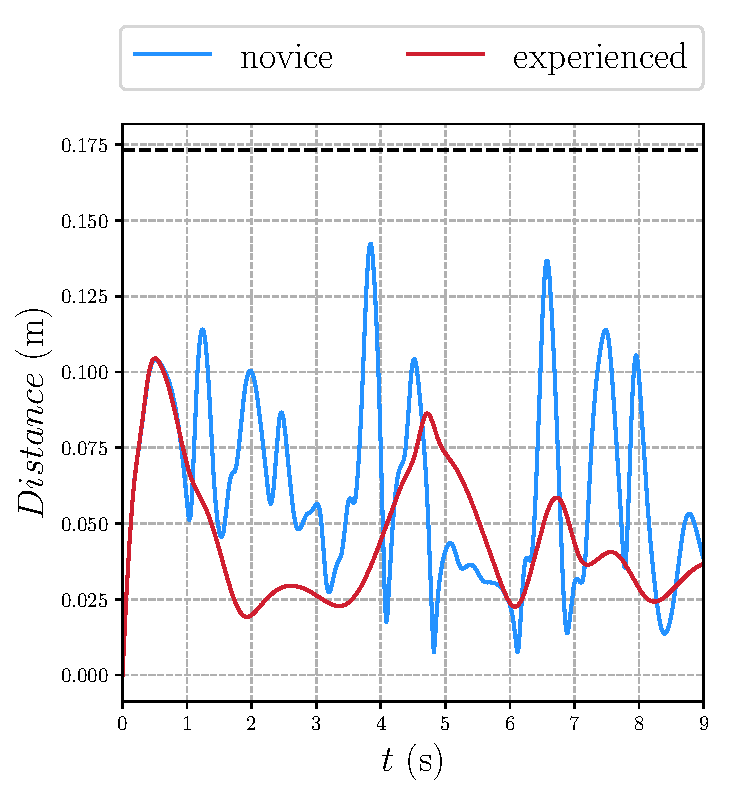
\includegraphics[width=0.4\textwidth]{figures/comparison}
	\vspace{-0.3cm}
	\caption{Distance between generated trajectories and reference; $\|\alpha\|$ is dashed.}\label{fig:boundary}%
\end{figure}
%===============================================================================
\begin{figure}[h]
	\centering
	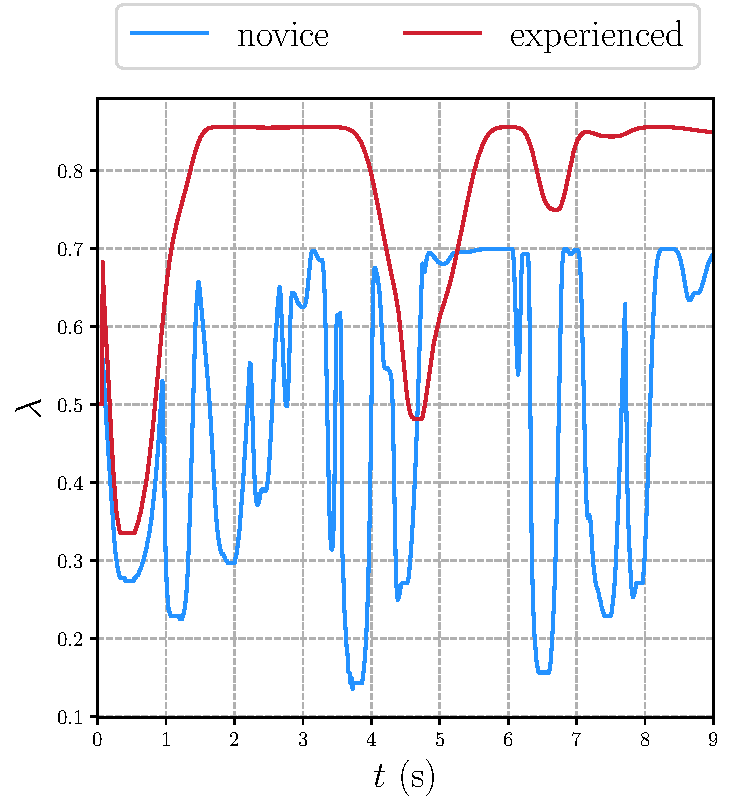
\includegraphics[width=0.38\textwidth]{figures/ph_index}
	\vspace{-0.3cm}
	\caption{Predicted healthiness index profiles indicating the level of human control authority.}\label{fig:ph_evo}%
\end{figure}
%===============================================================================
\begin{figure}[t]
	\centering
	\subfloat[Novice.]{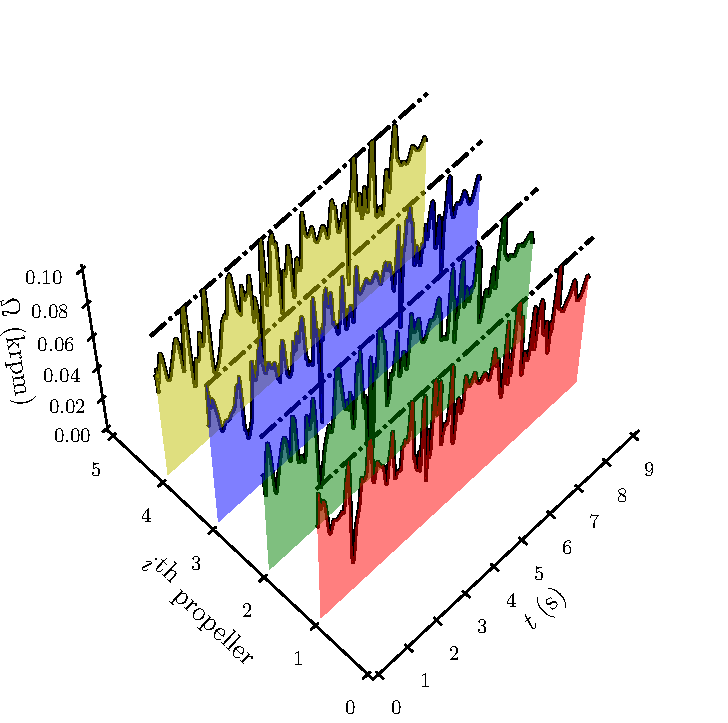
\includegraphics[width=0.4\textwidth]{figures/propeller_speed_novice}}\vspace{-0.39cm}
	\subfloat[Experienced.]{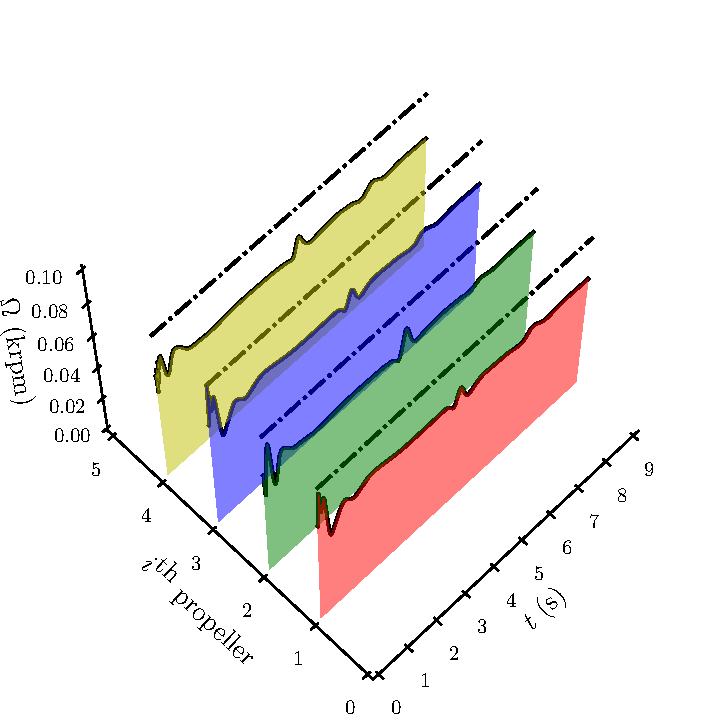
\includegraphics[width=0.4\textwidth]{figures/propeller_speed_experienced}}
	\caption{Generated propeller speeds; the upper bound $\bar{\Omega}$ is dashed.}\label{fig:prop_speed}%
\end{figure}
%===============================================================================
The proposed algorithm, that is, the blending mechanism and the mixed-initiative NMPC, use the parameters reported in Table \ref{tab:scenario1} in all test cases. In particular, we adopt a short virtual horizon $N_b$ to compensate for the fact that with a ZOH method, pilot inputs would have a natural tendency to violate the norm ball's boundary in the long run. The chosen value is a compromise between the base level of ``trust'' in the human inputs and the switching frequency of control authority. Another assumption made concerns the initialization of the blending mechanism. We assume that during the first iterations $\lambda = 0.5$, notably, none of the agents has control authority. Furthermore, the tests consider pilots with different competence levels. More specifically, the autonomous algorithm emulates a novice and an experienced pilot. This will enable a thorough follow-on comparative analysis of the control algorithm.    

Fig.~\ref{fig:output} displays the trajectories generated by our mixed-initiative NMPC for both pilots. The results show that our controller was able to maintain the quadrotor inside $\mathcal{B}$, successfully avoiding all obstacles in all cases (see Fig.~\ref{fig:boundary}). In Fig.~\ref{fig:human_inputs_s1}, we observe that the mixed-initiative NMPC commands closely follow the pilot inputs when the safety constraint is unlikely to be violated. This outcome is more evident for the experienced pilot, where the lines overlap almost completely, implying that the inputs issued kept the quadrotor closer to the reference trajectory. From Fig. \ref{fig:ph_evo}, it is obvious that the blending mechanism begins to drop off rapidly the level of control authority for the novice. At the same time, it maintains a relatively high level for the experienced pilot. Overall, note that the control algorithm assists the novice through what is often a very challenging part of their learning journey, the damping in pitching-rolling motions. The algorithm can keep up considerably with the signals' pattern (preserving the pilot's primary intentions), but attenuates their magnitude to cope with the safety constraint. Also, as the physical constraints herein regarded are linear, they can be enforced very efficiently by the optimization algorithm, as shown in Fig.~\ref{fig:prop_speed}.

Including maximum deviations provides versatility in the quadrotor motion generation. First, it gives a certain level of spatial freedom so that the quadrotor can leverage the motion by exploiting its dynamics. Second, it similarly adds new degrees of freedom to the controller. From a theoretic point of view, the control objective of the mixed-initiative NMPC can be seen as a target set (in the space of the task variables) instead of a target point, since inside $\mathcal{B}$ there are no preferences between one point and another \cite{camacho2010}.

The findings here indicate that our algorithm provides pilots with more control authority without sacrificing safety or even exceeding the robot's physical limits. Therefore, it has the potential to become a standard assistive scheme that can lead to a future improvement in pilot decision-making performance.

%===============================================================================
\begin{table}[h]
\caption{Parameters used by the blending mechanism and the mixed-initiative NMPC}
\centering
\begin{tabular}{cc|cc}
\toprule
$\ubar{\Omega}$ & $0$ & $\Bar{\Omega}$ & $0.09$ kHz \\
$\ubar{u}$ & $-0.1285$ Nm &  $\Bar{u}$ & $0.1285$ Nm \\
$T$ & $0.75$ s & $N$ & $50$ \\
$\alpha$ & $0.1{\cdot}\mathbf{1_3}$ m  & $N_b$ & $10$ \\
$\mu_1$ & 0.99 & $\mu_2$ & 0.3\\
$\theta_2$ & 50 & $\zeta$ & $1{\cdot}10^{-13}$\\
\midrule
\multicolumn{4}{c}{$Q_{\eta} = Q_{\eta_N} = \text{blkdiag}(250{\cdot}\mathbf{I_2}, 300)$, $Q_{\nu} = Q_{\nu_N} = 4{\cdot}10^3{\cdot}\mathbf{I_6}$,}\\
\multicolumn{4}{c}{$Q_{e} = Q_{e_N} = \text{blkdiag}(10, 3{\cdot}\mathbf{I_5}, 10)$, $R = 70{\cdot}\mathbf{I_4}$}\\
\bottomrule
\end{tabular}\label{tab:scenario1}
\end{table}
%===============================================================================